\documentclass[../DS01.tex]{subfiles}%
\graphicspath{{./figures/}}%

% \subimport{/home/nora/Documents/Enseignement/Prepa/bpep/exercices/DS/titrage_CO2/}{sujet.tex}%

\begin{document}%
\section[32]"E"{Étude de quelques lentilles minces\ifcorrige{~\small\textit{(D'après IESSA 2022)}}}

\subsection{Lentille convergente de focale donnée}

\enonce{%
	On considère une lentille convergente $\Lc$ de centre optique O et de distance
	focale $f' = \SI{20}{cm}$. Elle est utilisée dans les conditions de
	\textsc{Gauss} sur un banc d'optique. Elle donne d'un objet A sur l'axe
	optique une image A\bp sur l'axe optique.
	\smallbreak
	Pour les trois questions suivantes~:
	\begin{itemize}
		\item Faire un schéma à l'échelle en utilisant les \textbf{trois rayons
			      primaires}~;
		\item Caractériser l'image (virtuelle ou réelle, droite ou renversée,
		      agrandie, de même taille ou rétrécie)~;
		\item Déterminer par le calcul la position de l'image~;
		\item Calculer le grandissement.
	\end{itemize}
}%

\QR[8]{%
	On considère un objet réel AB perpendiculaire à l'axe optique et placé
	à \SI{40}{cm} de la lentille.
}{%
	\noindent
	\begin{minipage}[t]{.48\linewidth}
		On obtient donc une image \xul{réelle}, \xul{renversée} et de
		\xul{même taille} \pt{1} que l'objet. Avec la relation de
		\textsc{Descartes}~:
		\begin{gather*}
			\frac{1}{f'} \stm{=} \frac{1}{\OAp}-\frac{1}{\OA}
			\\\Lra
			\frac{1}{\OAp} = \frac{1}{\OA}+\frac{1}{f'}= \frac{\OA+f'}{\OA f'}
			\\\Lra
			\boxed{\OAp \stm{=} \frac{\OA f'}{\OA+f'}}
			\qav
			\left\{
			\begin{array}{rcl}
				\OA & = & \SI{-40}{cm}
				\\
				f'  & = & \SI{20}{cm}
			\end{array}
			\right.\\
			\AN
			\xul{
				\OAp \stm{=} \SI{40}{cm}
			}
		\end{gather*}
		De plus,
		\begin{gather*}
			\boxed{\gamma \stm{=} \frac{\OAp}{\OA}}
			\qav
			\left\{
			\begin{array}{rcl}
				\OAp & = & \SI{40}{cm}
				\\
				\OA  & = & \SI{-20}{cm}
			\end{array}
			\right.\\
			\AN
			\xul{
				\gamma \stm{=} -1
			}
		\end{gather*}
	\end{minipage}
	\hfill
	\begin{minipage}[t]{.48\linewidth}
		~
		\begin{center}
			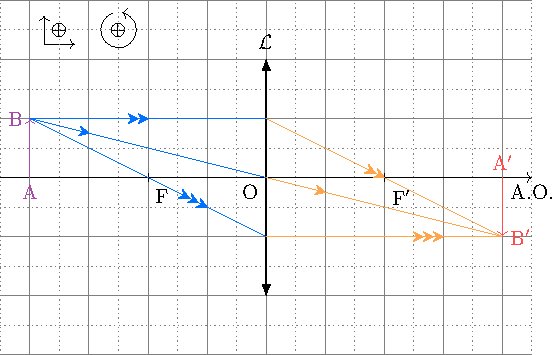
\includegraphics[width=\linewidth]{convAF}
			\captionof{figure}{\protect\pt{1}+\protect\pt{1}}
		\end{center}
	\end{minipage}
}%

\QR[5]{%
	On considère un objet réel AB perpendiculaire à l'axe optique et
	placé à \SI{10}{cm} de la lentille.
}{%
	\noindent
	\begin{minipage}[t]{.48\linewidth}
		On obtient donc une image \xul{virtuelle}, \xul{droite} et
		\xul{agrandie}. \pt{1} Avec la relation de \textsc{Descartes}~:
		\begin{gather*}
			\boxed{\OAp = \frac{\OA f'}{\OA+f'}}
			\qav
			\left\{
			\begin{array}{rcl}
				\OA & = & \SI{-10}{cm}
				\\
				f'  & = & \SI{20}{cm}
			\end{array}
			\right.\\
			\AN
			\xul{
				\OAp \stm{=} \SI{-20}{cm}
			}
		\end{gather*}
		De plus,
		\begin{gather*}
			\boxed{\gamma = \frac{\OAp}{\OA}}
			\qav
			\left\{
			\begin{array}{rcl}
				\OAp & = & \SI{-20}{cm}
				\\
				\OA  & = & \SI{-10}{cm}
			\end{array}
			\right.\\
			\AN
			\xul{
				\gamma \stm{=} +2
			}
		\end{gather*}
	\end{minipage}
	\hfill
	\begin{minipage}[t]{.48\linewidth}
		~
		\begin{center}
			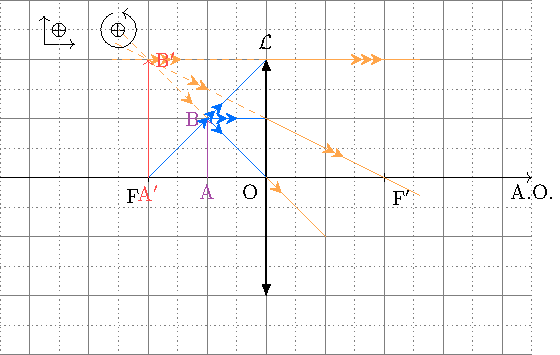
\includegraphics[width=\linewidth]{convCF}
			\captionof{figure}{\protect\pt{1}+\protect\pt{1}}
		\end{center}
	\end{minipage}
}%

\QR[5]{%
	On considère un objet virtuel AB perpendiculaire à l'axe optique et
	placé à \SI{20}{cm} de la lentille.
}{%
	\noindent
	\begin{minipage}[t]{.48\linewidth}
		On obtient donc une image \xul{réelle}, \xul{droite} et
		\xul{rétrécie}. \pt{1} Avec la relation de \textsc{Descartes}~:

		\begin{gather*}
			\boxed{\OAp = \frac{\OA f'}{\OA+f'}}
			\qav
			\left\{
			\begin{array}{rcl}
				\OA & = & \SI{20}{cm}
				\\
				f'  & = & \SI{20}{cm}
			\end{array}
			\right.\\
			\AN
			\xul{
				\OAp \stm{=} \SI{10}{cm}
			}
		\end{gather*}
		De plus,
		\begin{gather*}
			\boxed{\gamma = \frac{\OAp}{\OA}}
			\qav
			\left\{
			\begin{array}{rcl}
				\OAp & = & \SI{10}{cm}
				\\
				\OA  & = & \SI{20}{cm}
			\end{array}
			\right.\\
			\AN
			\xul{
				\gamma \stm{=} +0.5
			}
		\end{gather*}
	\end{minipage}
	\hfill
	\begin{minipage}[t]{.48\linewidth}
		~
		\begin{center}
			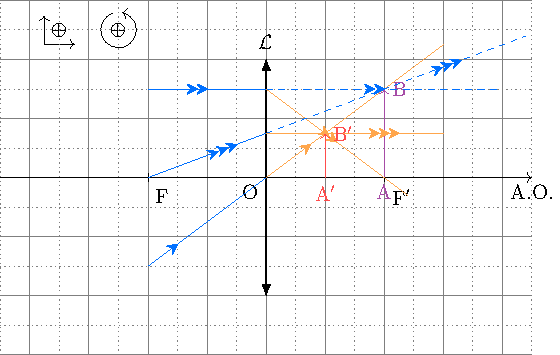
\includegraphics[width=\linewidth]{convDF}
			\captionof{figure}{\protect\pt{1}+\protect\pt{1}}
		\end{center}
	\end{minipage}
}%

\subsection{Lentille convergente quelconque}
\QR[3]{%
	Dans ce cas, l'image d'un objet réel est-elle toujours réelle~?
	Toujours virtuelle~? Ou aucune de ces deux affirmations n'est
	correcte~? Justifier.
}{%
	Les questions 1 et 2 montrent que pour un objet réel, une lentille
	convergente peut donner aussi bien une image réelle \pt{1} (question~1) que
	virtuelle (question~2). \pt{1} Donc pour l'image d'un objet réel à travers
	une lentille convergente, les deux cas peuvent se présenter. \pt{1}
}%

\QR[5]{%
	L'image d'un objet virtuel est-elle toujours réelle~? Toujours virtuelle~? Ou
	aucune de ces deux affirmations n'est correcte~? Justifier.
}{%
	Nous avons vu qu'avec la relation de \textsc{Descartes}, en isolant
	$\OAp$ on obtenait
	\[
		\OAp \stm{=} \frac{\OA f'}{\OA + f'}
	\]
	Si l'objet est virtuel, alors $\OA > 0$. \pt{1} Or, la lentille est
	convergente, donc $f' > 0$. \pt{1} Ainsi, $\OAp > 0$. \pt{1} En conclusion,
	l'image d'un objet virtuel au travers d'une lentille convergente est
	\xul{toujours réelle}. \pt{1}
}%

\subsection{Lentille divergente quelconque}
\QR[4]{%
	Dans ce cas, l'image d'un objet réel est-elle toujours réelle~? Toujours
	virtuelle~? Ou aucune de ces deux affirmations n'est correcte~? Justifier.
}{%
	De même que précédemment, le calcul de $\OAp$ avec un objet réel ($\OA
		< 0$ \pt{1}) pour une lentille divergente ($f' < 0$ \pt{1}) implique que
	$\OAp <
		0$. \pt{1} Ainsi, l'image d'un objet réel à travers une lentille divergente
	est donc \xul{toujours virtuelle}. \pt{1}
}%

\QR[2]{%
	L'image d'un objet virtuel est-elle toujours réelle~? Toujours
	virtuelle~? Ou aucune de ces deux affirmations n'est correcte~?
	Justifier.
}{%
	Cette fois, si $\OA > 0$ et $f' < 0$, alors $\OAp$ peut changer de
	signe selon les valeurs de $\OA$ et $f'$~: le produit est toujours
	négatif, mais $\OA + f' > 0$ si $\OA > -f'$ et inversement. \pt{1}
	\smallbreak
	Ainsi, pour un objet virtuel au travers d'une lentille divergente,
	\xul{les deux cas peuvent se présenter}. \pt{1}
	\begin{figure}[htbp]
		\centering
		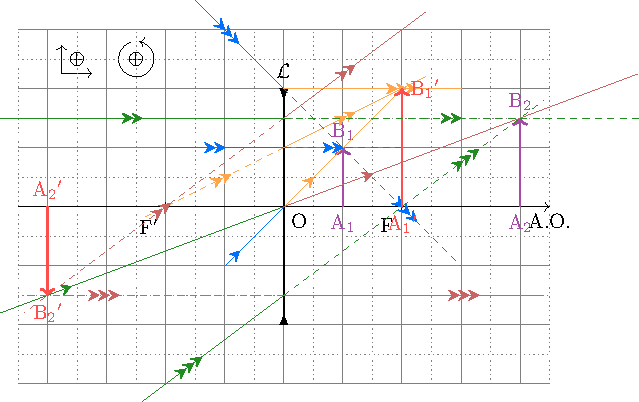
\includegraphics[width=.6\linewidth]{divCF}
		\caption{Image réelle ou virtuelle pour une lentille divergente.}
		\label{fig:divcf}
	\end{figure}
}%

\newpage

\end{document}
